\chapter{Matriisit}

Matriisi on kaksiulotteinen taulukko,
jolle on määritelty laskutoimituksia.
Tässä luvussa näemme, miten matriisien
avulla voi optimoida dynaamista ohjelmointia.
Osoittautuu, että jos dynaamisen ohjelmoinnin rekursiossa
lasketaan yhteen kiinteä määrä aiempia arvoja
vakiokertoimilla,

\section{Käsitteitä}

Olkoon $M$ matriisi, jonka koko on $n \times m$,
missä $n$ on korkeus (rivien määrä)
ja $m$ on leveys (sarakkeiden määrä).
Merkintä $M[i,j]$ tarkoittaa matriisin alkiota,
joka on rivillä $i$ sarakkeessa $j$,
kun $1 \le i \le n$ ja $1 \le j \le m$.

Esimerkiksi matriisin
\[
M = 
 \begin{bmatrix}
  6 & 13 & 7 & 4 \\
  7 & 0 & 8 & 2 \\
  9 & 5 & 4 & 18 \\
 \end{bmatrix}
\]

koko on $3 \times 4$,
eli sen korkeus on 3 ja leveys on 4.
Esimerkiksi $M[2,3]=8$,
koska rivillä 2 sarakkeessa 3
on luku 8.

Matriisin $M$ \textit{transpoosi} $M^T$ syntyy,
kun matriisin rivit ja sarakkeet vaihdetaan keskenään
eli $M^T[i,j]=M[j,i]$.
Esimerkiksi yllä olevan matriisin transpoosi
on seuraava:
\[
M^T = 
 \begin{bmatrix}
  6 & 7 & 9 \\
  13 & 0 & 5 \\
  7 & 8 & 4 \\
  4 & 2 & 18 \\
 \end{bmatrix}
\]

Matriisi $M$ on \textit{neliömatriisi}, jos matriisi
on kokoa $n \times n$ eli sen korkeus ja leveys ovat samat.
Esimerkiksi seuraava matriisi on neliömatriisi:

\[
M = 
 \begin{bmatrix}
  3 & 12 & 4  \\
  5 & 9 & 15  \\
  0 & 2 & 4 \\
 \end{bmatrix}
\]

\subsubsection{Matriisisumma}

Matriisien $A$ ja $B$ summa $A+B$ on määritelty,
jos matriisit ovat yhtä suuret.
Tuloksena oleva summamatriisi $S$ on yhtä suuri kuin
matriisit $A$ ja $B$ ja sen alkiot
lasketaan kaavalla

\[ S[i,j]=A[i,j]+B[i,j]. \]

Esimerkiksi

\[
 \begin{bmatrix}
  6 & 1 & 4 \\
  3 & 9 & 2 \\
 \end{bmatrix}
+
 \begin{bmatrix}
  4 & 9 & 3 \\
  8 & 1 & 3 \\
 \end{bmatrix}
=
 \begin{bmatrix}
  6+4 & 1+9 & 4+3 \\
  3+8 & 9+1 & 2+3 \\
 \end{bmatrix}
=
 \begin{bmatrix}
  10 & 10 & 7 \\
  11 & 10 & 5 \\
 \end{bmatrix}.
\]
Matriisisumma on vaihdannainen ja liitännäinen,
eli pätee $A+B=B+A$ ja $A+(B+C)=(A+B)+C$.
% Lukua 0 vastaa nollamatriisi $O$,
% jolle pätee $M+O=M$ ja $O+M=M$.
% Nollamatriisin jokainen alkio on 0.
% Esimerkiksi
% 
% \[
%  \begin{bmatrix}
%   6 & 1 & 4 \\
%   3 & 9 & 2 \\
%  \end{bmatrix}
% +
%  \begin{bmatrix}
%   0 & 0 & 0 \\
%   0 & 0 & 0 \\
%  \end{bmatrix}
% =
%  \begin{bmatrix}
%   6 & 1 & 4 \\
%   3 & 9 & 2 \\
%  \end{bmatrix}.
% \]

\subsubsection{Matriisitulo}

Matriisien $A$ ja $B$ tulo $A \cdot B$ on määritelty,
jos matriisi $A$ on kokoa $a \times n$
ja matriisi $B$ on kokoa $n \times b$,
eli matriisin $A$ leveys on sama kuin matriisin
$B$ korkeus.
Tulomatriisi $T$
on kokoa $a \times b$
ja sen alkiot lasketaan kaavalla
\[
T[i,j] = \sum_{k=1}^n A[i,k] \cdot B[k,j].
\]

Kaavan tulkintana on, että kukin $T$:n alkio
saadaan summana, joka muodostuu $A$:n ja
$B$:n alkioparien tuloista seuraavan
kuvan mukaisesti:

\begin{center}
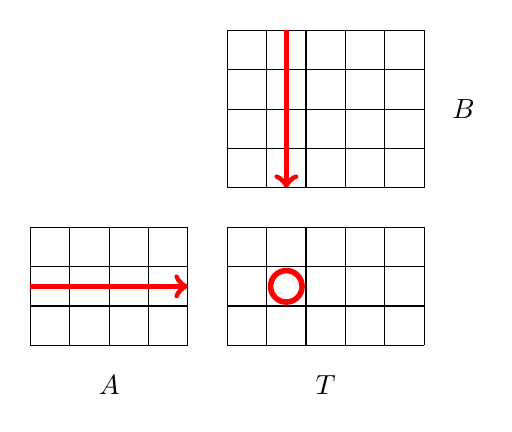
\begin{tikzpicture}[scale=0.5]
\draw (0,0) grid (4,3);
\draw (5,0) grid (10,3);
\draw (5,4) grid (10,8);

\node at (2,-1) {$A$};
\node at (7.5,-1) {$T$};
\node at (11,6) {$B$};

\draw[thick,->,red,line width=2pt] (0,1.5) -- (4,1.5);
\draw[thick,->,red,line width=2pt] (6.5,8) -- (6.5,4);
\draw[thick,red,line width=2pt] (6.5,1.5) circle (0.4);
\end{tikzpicture}
\end{center}

Esimerkiksi

\[
 \begin{bmatrix}
  1 & 4 \\
  3 & 9 \\
  8 & 6 \\
 \end{bmatrix}
\cdot
 \begin{bmatrix}
  1 & 6 \\
  2 & 9 \\
 \end{bmatrix}
=
 \begin{bmatrix}
  1 \cdot 1 + 4 \cdot 2 & 1 \cdot 6 + 4 \cdot 9 \\
  3 \cdot 1 + 9 \cdot 2 & 3 \cdot 6 + 9 \cdot 9 \\
  8 \cdot 1 + 6 \cdot 2 & 8 \cdot 6 + 6 \cdot 9 \\
 \end{bmatrix}
=
 \begin{bmatrix}
  9 & 42 \\
  21 & 99 \\
  20 & 102 \\
 \end{bmatrix}.
\]

Matriisitulo ei ole vaihdannainen,
eli ei ole voimassa $A \cdot B = B \cdot A$.
Kuitenkin matriisitulo
on liitännäinen, eli on voimassa $A \cdot (B \cdot C)=(A \cdot B) \cdot C$.

\textit{Ykkösmatriisi} on neliömatriisi,
jonka lävistäjän jokainen alkio on 1
ja jokainen muu alkio on 0.
Esimerkiksi $3 \times 3$ -yksikkömatriisi on
seuraavanlainen:
\[
 \begin{bmatrix}
  1 & 0 & 0 \\
  0 & 1 & 0 \\
  0 & 0 & 1 \\
 \end{bmatrix}
\]

Ykkösmatriisilla kertominen säilyttää matriisin
ennallaan. Esimerkiksi

\[
 \begin{bmatrix}
  1 & 0 & 0 \\
  0 & 1 & 0 \\
  0 & 0 & 1 \\
 \end{bmatrix}
\cdot
 \begin{bmatrix}
  1 & 4 \\
  3 & 9 \\
  8 & 6 \\
 \end{bmatrix}
=
 \begin{bmatrix}
  1 & 4 \\
  3 & 9 \\
  8 & 6 \\
 \end{bmatrix} \hspace{10px} \textrm{ja} \hspace{10px}
 \begin{bmatrix}
  1 & 4 \\
  3 & 9 \\
  8 & 6 \\
 \end{bmatrix}
\cdot
 \begin{bmatrix}
  1 & 0 \\
  0 & 1 \\
 \end{bmatrix}
=
 \begin{bmatrix}
  1 & 4 \\
  3 & 9 \\
  8 & 6 \\
 \end{bmatrix}.
\]

Matriisitulon määritelmästä seuraa kuutiollinen
algoritmi, joka on riittävän nopea kisakoodauksessa:

\begin{lstlisting}
for (int i = 1; i <= a; i++) {
    for (int j = 1; j <= b; j++) {
        for (int k = 1; k <= n; k++) {
            T[i][j] += A[i][k]*B[k][j];
        }
    }
}
\end{lstlisting}

\subsubsection{Matriisipotenssi}

Matriisin $M$ potenssi $M^k$ on
määritelty, jos $M$ on neliömatriisi.
Määritelmä nojautuu kertolaskuun:
\[ M^k = \underbrace{M \cdot M \cdot M \cdots M}_{\textrm{$k$ kertaa}} \]
Esimerkiksi

\[
 \begin{bmatrix}
  2 & 5 \\
  1 & 4 \\
 \end{bmatrix}^3 =
 \begin{bmatrix}
  2 & 5 \\
  1 & 4 \\
 \end{bmatrix} \cdot
 \begin{bmatrix}
  2 & 5 \\
  1 & 4 \\
 \end{bmatrix} \cdot
 \begin{bmatrix}
  2 & 5 \\
  1 & 4 \\
 \end{bmatrix} =
 \begin{bmatrix}
  48 & 165 \\
  33 & 114 \\
 \end{bmatrix}.
\]
Lisäksi $M^0$ tuottaa ykkösmatriisin. Esimerkiksi
\[
 \begin{bmatrix}
  2 & 5 \\
  1 & 4 \\
 \end{bmatrix}^0 =
 \begin{bmatrix}
  1 & 0 \\
  0 & 1 \\
 \end{bmatrix}.
\]

Matriisin $M^k$ voi laskea tehokkaasti ajassa
$O(n^3 \log k)$ soveltamalla luvun 21.2
tehokasta potenssilaskua. Esimerkiksi
\[
 \begin{bmatrix}
  2 & 5 \\
  1 & 4 \\
 \end{bmatrix}^8 =
 \begin{bmatrix}
  2 & 5 \\
  1 & 4 \\
 \end{bmatrix}^4 \cdot
 \begin{bmatrix}
  2 & 5 \\
  1 & 4 \\
 \end{bmatrix}^4.
\]


\subsubsection{Determinantti}

Matriisin $A$ \textit{determinantti} $\det(A)$
on määritelty, jos $A$ on neliömatriisi.
Jos $A$ on kokoa $1 \times 1$,
niin $\det(A)=A[1,1]$.
Muuten determinaatti lasketaan rekursiivisesti
kaavalla

\[\det(A)=\sum_{i=1}^n A[1,i] \cdot det(A') \cdot (-1)^{i+1},\]

missä $A'$ tarkoittaa matriisia $A$,
josta on poistettu rivi 1 ja sarake $i$.
Huomaa myös, että $(-1)^{i+1}$ on $1$,
jos $i$ on pariton, ja muuten $-1$.

Esimerkiksi

\[
\det(
 \begin{bmatrix}
  3 & 4 \\
  1 & 6 \\
 \end{bmatrix}
) = 3 \cdot 6 - 4 \cdot 1 = 14 
\]

ja

\[
\det(
 \begin{bmatrix}
  2 & 4 & 3 \\
  5 & 1 & 6 \\
  7 & 2 & 4 \\
 \end{bmatrix}
) = 
2 \cdot
\det(
 \begin{bmatrix}
  1 & 6 \\
  2 & 4 \\
 \end{bmatrix}
)
-4 \cdot
\det(
 \begin{bmatrix}
  5 & 6 \\
  7 & 4 \\
 \end{bmatrix}
)
+3 \cdot
\det(
 \begin{bmatrix}
  5 & 1 \\
  7 & 2 \\
 \end{bmatrix}
) = 81.
\]

Determinantti kertoo, onko matriisille
$A$ olemassa käänteismatriisia
$A^{-1}$, jolle pätee $A \cdot A^{-1} = I$.
Osoittautuu, että käänteismatriisi on olemassa
tarkalleen silloin, kun $\det(A) \neq 0$.
Esimerkiksi

\[
\underbrace{
 \begin{bmatrix}
  3 & 4 \\
  1 & 6 \\
 \end{bmatrix}
}_{A}
\cdot
\underbrace{
 \begin{bmatrix}
  \frac{3}{7} & -\frac{2}{7} \\
  -\frac{1}{14} & \frac{3}{14} \\
 \end{bmatrix}
}_{A^{-1}}
=
\underbrace{
 \begin{bmatrix}
  1 & 0 \\
  0 & 1 \\
 \end{bmatrix}
}_{I}.
\]

\section{Lineaariset rekursioyhtälöt}

Lineaarinen rekursioyhtälö 
voidaan esittää funktiona $f(n)$,
jolle on annettu alkuarvot
$f(0),f(1),\ldots,f(k-1)$
ja jonka suuremmat arvot
parametrista $k$ lähtien lasketaan
rekursiivisesti kaavalla
\[f(n) = c_1 f(n-1) + c_2 f(n-2) + \ldots + c_k f (n-k),\]
missä $c_1,c_2,\ldots,c_k$ ovat vakiokertoimia.

Funktion arvon $f(n)$ voi laskea dynaamisella
ohjelmoinnilla ajassa $O(kn)$
laskemalla kaikki arvot $f(0),f(1),\ldots,f(n)$ järjestyksessä.
Tätä ratkaisua voi kuitenkin tehostaa merkittävästi
matriisien avulla.
Opimme seuraavaksi, miten arvon $f(n)$
voi laskea ajassa $O(k^3 \log n)$.

\subsubsection{Fibonaccin luvut}

Yksinkertainen esimerkki lineaarisesta rekursioyhtälöstä
on Fibonaccin luvut määrittelevä funktio:
\[
\begin{array}{lcl}
f(0) & = & 0 \\
f(1) & = & 1 \\
f(n) & = & f(n-1)+f(n-2) \\
\end{array}
\]
Tässä tapauksessa $k=2$ ja $c_1=c_2=1$.

Ideana on esittää rekursiivinen kaava $k \times k$
-kokoisena neliömatriisina $X$, jolle pätee

\[ X \cdot
 \begin{bmatrix}
  f(i) \\
  f(i+1) \\
 \end{bmatrix}
=
 \begin{bmatrix}
  f(i+1) \\
  f(i+2) \\
 \end{bmatrix}.
 \]
Tämä tarkoittaa, että matriisille $X$ annetaan
''syötteenä'' $k$ peräkkäistä funktion $f$ arvoa
kohdasta $i$ alkaen ja kertolaskun tuloksena
on $k$ peräkkäistä arvoa kohdasta $i+1$ alkaen.
Fibonaccin lukujen tapauksessa tällainen matriisi on

\[ X = 
 \begin{bmatrix}
  0 & 1 \\
  1 & 1 \\
 \end{bmatrix}.
\]

Esimerkiksi

\[
 \begin{bmatrix}
  0 & 1 \\
  1 & 1 \\
 \end{bmatrix}
\cdot
 \begin{bmatrix}
  f(5) \\
  f(6) \\
 \end{bmatrix}
=
 \begin{bmatrix}
  0 & 1 \\
  1 & 1 \\
 \end{bmatrix}
\cdot
 \begin{bmatrix}
  5 \\
  8 \\
 \end{bmatrix}
=
 \begin{bmatrix}
  8 \\
  13 \\
 \end{bmatrix}
=
 \begin{bmatrix}
  f(6) \\
  f(7) \\
 \end{bmatrix}.
\]

Tämän ansiosta arvon $f(n)$ sisältävän matriisin saa laskettua
kaavalla

\[
 \begin{bmatrix}
  f(n) \\
  f(n+1) \\
 \end{bmatrix}
=
X^n \cdot
 \begin{bmatrix}
  f(0) \\
  f(1) \\
 \end{bmatrix}
=
 \begin{bmatrix}
  0 & 1 \\
  1 & 1 \\
 \end{bmatrix}^n
\cdot
 \begin{bmatrix}
  0 \\
  1 \\
 \end{bmatrix}.
\]

Potenssilasku $X^n$ onnistuu ajassa
$O(k^3 \log n)$,
joten myös funktion arvon $f(n)$
saa laskettua ajassa $O(k^3 \log n)$.

\subsubsection{Yleinen tapaus}

Tarkastellaan sitten yleistä tapausta,
missä $f(n)$ on mikä tahansa lineaarinen
rekursioyhtälö. Nyt tavoitteena on etsiä
matriisi $X$, jolle pätee

\[ X \cdot
 \begin{bmatrix}
  f(i) \\
  f(i+1) \\
  \vdots \\
  f(i+k-1) \\
 \end{bmatrix}
=
 \begin{bmatrix}
  f(i+1) \\
  f(i+2) \\
  \vdots \\
  f(i+k) \\
 \end{bmatrix}.
\]

Tällainen matriisi on

\[
X =
 \begin{bmatrix}
  0 & 1 & 0 & 0 & \cdots & 0 \\
  0 & 0 & 1 & 0 & \cdots & 0 \\
  0 & 0 & 0 & 1 & \cdots & 0 \\
  \vdots & \vdots & \vdots & \vdots & \ddots & \vdots \\
  0 & 0 & 0 & 0 & \cdots & 1 \\
  c_k & c_{k-1} & c_{k-2} & c_{k-3} & \cdots & c_1 \\
 \end{bmatrix}.
\]
Matriisin $k-1$ ensimmäisen rivin jokainen alkio on 0,
paitsi yksi alkio on 1.
Näiden rivien tarkoituksena on kopioida
arvo $f(i+1)$ arvon $f(i)$ tilalle,
arvo $f(i+2)$ arvon $f(i+1)$ tilalle jne.
Viimeinen rivi sisältää rekursiokaavan kertoimet,
joiden avulla muodostuu uusi arvo $f(i+k)$.

Nyt arvon $f(n)$ pystyy laskemaan ajassa $O(k^3 \log n)$
kaavalla

\[
 \begin{bmatrix}
  f(n) \\
  f(n+1) \\
  \vdots \\
  f(n+k-1) \\
 \end{bmatrix}
=
X^n \cdot
 \begin{bmatrix}
  f(0) \\
  f(1) \\
  \vdots \\
  f(k-1) \\
 \end{bmatrix}.
\]


\section{Verkkojen käsittely}

\subsection{Polkujen määrät}

Matriisipotenssilla
on mielenkiintoinen vaikutus
verkon vierusmatriisin sisältöön.
Kun $V$ on painottoman verkon vierusmatriisi,
niin $V^n$ kertoo,
montako $n$ kaaren pituista polkua
eri solmuista on toisiinsa.

Esimerkiksi verkon
\begin{center}
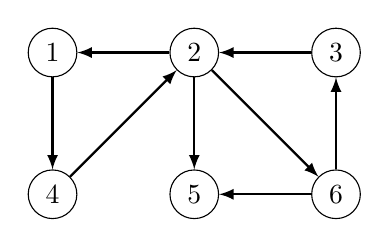
\begin{tikzpicture}[scale=0.9]
\node[draw, circle] (1) at (1,3) {$1$};
\node[draw, circle] (2) at (1,1) {$4$};
\node[draw, circle] (3) at (3,3) {$2$};
\node[draw, circle] (4) at (5,3) {$3$};
\node[draw, circle] (5) at (3,1) {$5$};
\node[draw, circle] (6) at (5,1) {$6$};

\path[draw,thick,->,>=latex] (1) -- (2);
\path[draw,thick,->,>=latex] (2) -- (3);
\path[draw,thick,->,>=latex] (3) -- (1);
\path[draw,thick,->,>=latex] (4) -- (3);
\path[draw,thick,->,>=latex] (3) -- (5);
\path[draw,thick,->,>=latex] (3) -- (6);
\path[draw,thick,->,>=latex] (6) -- (4);
\path[draw,thick,->,>=latex] (6) -- (5);
\end{tikzpicture}
\end{center}

vierusmatriisi on

\[
V= \begin{bmatrix}
  0 & 0 & 0 & 1 & 0 & 0 \\
  1 & 0 & 0 & 0 & 1 & 1 \\
  0 & 1 & 0 & 0 & 0 & 0 \\
  0 & 1 & 0 & 0 & 0 & 0 \\
  0 & 0 & 0 & 0 & 0 & 0 \\
  0 & 0 & 1 & 0 & 1 & 0 \\
 \end{bmatrix}.
\]

Nyt esimerkiksi matriisi
\[
V^4= \begin{bmatrix}
  0 & 0 & 1 & 1 & 1 & 0 \\
  2 & 0 & 0 & 0 & 2 & 2 \\
  0 & 2 & 0 & 0 & 0 & 0 \\
  0 & 2 & 0 & 0 & 0 & 0 \\
  0 & 0 & 0 & 0 & 0 & 0 \\
  0 & 0 & 1 & 1 & 1 & 0 \\
 \end{bmatrix}
\]

kertoo, montako 4 kaaren pituista polkua
solmuista on toisiinsa.
Esimerkiksi $V^4[2,5]=2$,
koska solmusta 2 solmuun 5 on olemassa
4 kaaren pituiset polut
$2 \rightarrow 1 \rightarrow 4 \rightarrow 2 \rightarrow 5$
ja 
$2 \rightarrow 6 \rightarrow 3 \rightarrow 2 \rightarrow 5$.

\subsection{Lyhimmät polut}

Samantapaisella idealla voi laskea painotetussa verkossa
kullekin solmuparille,
mikä on lyhin $n$ kaaren pituinen polku.
Tarkastellaan esimerkkinä seuraavaa verkkoa:

\begin{center}
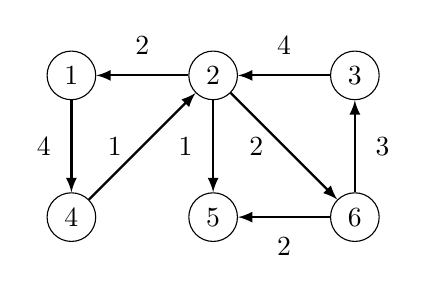
\begin{tikzpicture}[scale=0.9]
\node[draw, circle] (1) at (1,3) {$1$};
\node[draw, circle] (2) at (1,1) {$4$};
\node[draw, circle] (3) at (3,3) {$2$};
\node[draw, circle] (4) at (5,3) {$3$};
\node[draw, circle] (5) at (3,1) {$5$};
\node[draw, circle] (6) at (5,1) {$6$};

\path[draw,thick,->,>=latex] (1) -- node[font=\small,label=left:4] {} (2);
\path[draw,thick,->,>=latex] (2) -- node[font=\small,label=left:1] {} (3);
\path[draw,thick,->,>=latex] (3) -- node[font=\small,label=north:2] {} (1);
\path[draw,thick,->,>=latex] (4) -- node[font=\small,label=north:4] {} (3);
\path[draw,thick,->,>=latex] (3) -- node[font=\small,label=left:1] {} (5);
\path[draw,thick,->,>=latex] (3) -- node[font=\small,label=left:2] {} (6);
\path[draw,thick,->,>=latex] (6) -- node[font=\small,label=right:3] {} (4);
\path[draw,thick,->,>=latex] (6) -- node[font=\small,label=below:2] {} (5);
\end{tikzpicture}
\end{center}

Muodostetaan verkosta vierusmatriisi, jossa arvo
$\infty$ tarkoittaa, että kaarta ei ole,
ja muut arvot ovat kaarten pituuksia.
Matriisista tulee
\[
V= \begin{bmatrix}
  \infty & \infty & \infty & 4 & \infty & \infty \\
  2 & \infty & \infty & \infty & 1 & 2 \\
  \infty & 4 & \infty & \infty & \infty & \infty \\
  \infty & 1 & \infty & \infty & \infty & \infty \\
  \infty & \infty & \infty & \infty & \infty & \infty \\
  \infty & \infty & 3 & \infty & 2 & \infty \\
 \end{bmatrix}.
\]

Nyt ideana on laskea matriisitulo kaavan
\[
AB[i,j] = \sum_{k=1}^n A[i,k] \cdot B[k,j]
\]
sijasta kaavalla
\[
AB[i,j] = \min_{k=1}^n A[i,k] + B[k,j],
\]
eli summa muuttuu minimiksi ja tulo summaksi.
Tämän seurauksena matriisipotenssi
selvittää lyhimmät polkujen pituudet solmujen
välillä. Esimerkiksi

\[
V^4= \begin{bmatrix}
  \infty & \infty & 10 & 11 & 9 & \infty \\
  9 & \infty & \infty & \infty & 8 & 9 \\
  \infty & 11 & \infty & \infty & \infty & \infty \\
  \infty & 8 & \infty & \infty & \infty & \infty \\
  \infty & \infty & \infty & \infty & \infty & \infty \\
  \infty & \infty & 12 & 13 & 11 & \infty \\
 \end{bmatrix}
\]
eli esimerkiksi lyhin 4 kaaren pituinen polku
solmusta 2 solmuun 5 on pituudeltaan 8.
Tämä polku on $2 \rightarrow 1 \rightarrow 4 \rightarrow 2 \rightarrow 5$.


\subsection{Kirchhoffin lause}



